\documentclass[11pt,letterpaper]{article}
\usepackage[top=1in,bottom=1in,left=1in,right=1in]{geometry}
\usepackage[numbers]{natbib}      % http://merkel.zoneo.net/Latex/natbib.php
\usepackage{palatino}
\bibpunct{(}{)}{;}{a}{,}{,}
\usepackage{chngpage}
\usepackage{stmaryrd}
\usepackage{amssymb}
\usepackage{amsmath}
\usepackage{amsthm}
\usepackage{graphicx}
\usepackage{lscape}
\usepackage{subfigure}
\usepackage{parskip}
\usepackage{float}
\usepackage[usenames,dvipsnames]{color}
\usepackage{indentfirst}
\definecolor{myblue}{rgb}{0,0.1,0.6}
\definecolor{mygreen}{rgb}{0,0.3,0.1}
\usepackage[colorlinks=true,linkcolor=black,citecolor=mygreen,urlcolor=myblue]{hyperref}

\newcommand\norm[1]{\left\lVert#1\right\rVert}
\newcommand{\ignore}[1]{}

\setlength{\parindent}{30pt}
\linespread{1}

\title{
	Regularization\footnote{This material is for self-study only.}
}

\author{
	Khanh Nguyen
}

\date{June 14, 2015}

\begin{document}
\maketitle

\section{Overview}

Overfitting is a persistent problem in machine learning. Although, in most cases, training machine learning models requires maximizing the likelihood of training data, the ultimate goal is about making the model be able to generalize its predictive capability to unseen data. Therefore, if the training objective function consists of only the likelihood of the training dataset, the model will perform poorly on an unseen dataset if its distribution is different from the training set. This phenomenon is known as \emph{overfitting}. From a different perspective, overfitting is the case when the model's variance is high, i.e. it alters dramatically on different datasets. 

To avoid overfitting, a model should be given information beyond its training dataset. Hence, the general purpose of regularization methods is to inject \emph{inductive bias} into the model. For example,
\begin{itemize}
\item Prevent the training algorithm from picking undesirable parameters (e.g. all-zero or overflowed parameters). 
\item Direct the training algorithm to picking desirable parameters (e.g. sparse parameters).  
\item Represent the prior(s) of the data generating process. This prior acts as a list of preference scores over all parameter configurations. This is the generalization of the two points above.
\end{itemize}

Regularization can be achieved by several ways. One of the most popular forms of regularization is called \emph{regularization penalty}.  In this case, an extra term that is dependent on the model parameters  is added to the training objective. This term is then trained jointly with the log likelihood of the training data. There is also a regularization strength constant to control the degree of regularization. Regularization penalty is successfully used in many classic models such as logistic regression or conditional random fields. However, there are two major drawbacks with this approach: (a) non-smooth regularization terms might hinder optimization; (b) tuning the regularization strength requires training the model many times. Hence, it is not very suitable for non-convex and complex models such as large-scaled neural networks. Modern approach on regularization for these types of models involves techniques that do not modify the training objective. Two most common ones are \emph{early stopping} and \emph{dropout}. At first, they are not intuitively recognized as regularization techniques. However, their effects on the controlling model parameters has been shown. For example, one can show that early stopping in linear regression is equivalent to L2-regularization. Moreover, they are easy to implement but still efficient in practice. 

In this note, I will discuss all of those regularization methods mentioned so far. This material is largely based on the book \emph{Deep Learning} by Yoshua Bengio, Ian J. Goodfellow and Aaron Courville, and the book \emph{Machine Learning: A Probabilistic Perspective} by Kevin Murphy. 

\section{L2-regularization}

The L2-regularizer, also known as weight decay, penalizes the training objective by a norm-2 of the parameter vector (or the weight vector) $w$:
$$
J(w) = NLL(w) + \frac{1}{2} \alpha \norm{w}_2
$$ where NLL(w) is the negative log-likelihood of the training data, $\norm{w}_2 = \sum_i w_i^2$ is the norm-2 of the parameter vector $w$, and $\alpha$ is the regularization strength \footnote{Notice that to penalize the objective, we have to "add" the regularizer since the goal is to minimize the objective.}.

The gradient of the object with respect to $w$ is:
\begin{equation}
 \nabla J(w) = \nabla_w NLL(w) + \alpha w
\end{equation}

Consider a quadratic approximation of the negative log-likelihood near the neighborhood of the optimal value parameters $w^*$:
$$ \hat{NLL}(w) = NLL(w^*) + \frac{1}{2}(w - w^*)^T H(w - w^*)$$ where $H$ is the Hessian matrix of $NLL(w)$ with respect to $w$ \footnote{The gradient term does not appear since $w^*$ is an optimum.}.

Then, 
\begin{equation}
\nabla \hat{NLL}_w(w) = H(w - w^*)
\end{equation}

Replace $\nabla_w NLL(w)$ in (1) by the approximation in (2) and set the gradient to be zero, we have:
$$ H(w - w^*) + \alpha w = 0$$
or
$$
w = (H + \alpha I)^{-1}Hw^*
$$

We observe the followings from the above equation:
\begin{itemize}
\item As $\lambda$ goes to, $w$ approaches its optimal value $w^*$ as when training with the log-likelihood only. 

\item Since $H$ is symmetric, $H = Q \Lambda Q^T$, for some orthonormal matrix $Q$ and some diagonal matrix $\Lambda$. Then:
$$ w = Q(\Lambda + \alpha I)^{-1} \Lambda Q^T w^*$$
We interpret the left hand side as rotating $w*$ to the space spanned by the eigenvectors of $H$, scaling each component $i$ by a factor of $\frac{\lambda_i}{\lambda _i + \alpha}$, then rotating it back to the original space. This explains the name \emph{weight decay}. Each component of the parameters is suppressed. The strength of suppression varies depending on the magnitude of each component. Particularly, when $\lambda_i$ is negligible, the $\alpha$ term in the denominator will dominate and scale the  corresponding component to almost zero. Hence, the model will be more likely to go with a set of small-valued parameters. As a result, the variance of the parameters is limited to a smaller range so overfitting will be mitigated.


\end{itemize}


From a Bayesian perspective, L2-regularization can be interpreted as placing a Gaussian prior with mean zero on theparamters. The reguarization strength is related to the variance of that Gaussian distribution. Since the Gaussian concentrates its mass on values near zeros, the Gaussian prior represents a preference for small-valued parameters.  
\section{L1-regularization}

L1-regularization also limits the variance of the model. It achieves that effect in a slightly different way from L2-regularization. Interestingly, the parameter vector of a model trained by a L1-regularized objective is often sparse, i.e. contains mostly zero entries. 

An L1-regularized objective takes the form:
$$
J(w) = NLL(w) + \alpha \norm{w}_1
$$ where NLL(w) is the negative log-likelihood of the training data and $\norm{w}_1 = \sum_i |w_i|$ is the norm-1 of the parameter vector $w$, and $\alpha$ is the regularization strength.

The sub-gradient with respect to $w$ is:

$$ \nabla_w J(w) = \nabla NLL(w) + \alpha \ \text{sign}(w) $$ where sign(w) returns a vector that contains the signs of elements of $w$. 

As for L2-regularization, the penalty for each component of $w$ varies depending on the magnitude of that component. In the case of L1-regularization, however, each component is penalized by the same amount, plus or minus the regularization strength. This means smaller components will be pushed harder towards zero than greater components are.   

There are several ways to understand the behavior of the L1-regularization. First of all, let's think of its as introducing a Laplace prior on the parameter vector. Recall that L2-regularization can be interpreted as a Gaussian prior. The main difference between the Guassian distribution and the Laplace distribution that is that the latter tends to be more heavy-tailed and allocate more probability mass at zero. In particular, we can visualize the difference function between these two type of regularizations in a 2D least square problem (Figure \ref{fig:l1vsl2} \footnote{Picture taken from Kevin Murphy's \emph{Machine Learning: a Probabilistic Approach}, page 430.}).

\begin{figure}[H]
\centering
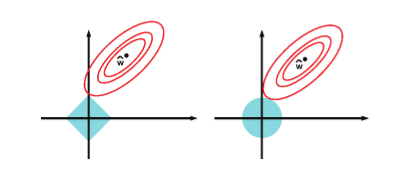
\includegraphics[width=0.6\textwidth]{l1vsl2.png}
\caption{(a) L1 (b) L2}
\label{fig:l1vsl2}
\end{figure}

A regularized solution for this problem will lie at the intersection of the blue area and the red contour. As we can see, the blue area for L1-regularization is less inflated; hence, the red contour is more likely to touch it at points where the parameters are sparse. 

\section{Early stopping}

Recall that overfitting occurs when the generalization error starts to increase while the training error keeps descreasing. Therefore, to avoid overfitting, it is very natural to simply stop training as soon as we encounter this phenomenon. This is called \emph{early stopping}. More generally, we should use the set of parameters that gives the best performance on the validation set. 

One can show that early stopping for linear model with a quadratic loss function is equivalance to L2-regularization \footnote{see the section on regularization of Bengio et al.'s \emph{Deep Learning} book}. The number of training steps is closely related to the regularization strength in that case.

The most appealing aspect of early stopping is its simplicity. It does not the require re-engineering the loss function, which would lead to non-smooth or non-convex function and hinders optimization. Moreover, since the only hyper-parameter for early stopping is number of training steps, it does not require re-training the model to pick the optimal hyper-parameters. On the other hand, selecting the optimal hyper-parameter for L1 or L2 regularization is a very time-consuming process. There is a pitfall for early stopping though. A extra validation set will be needed, which is not always the case for many problems. In addition, when training the final version of a model, we would want to combine the validation set with the training set together. Then in that case it is unclear what the number of steps we would train the model on the new dataset should be.   

\section{Dropout}

\emph{Dropout} is a very effective regularization technique in deep learning. The motivation for dropout is another technique called \emph{bagging}, i.e. having many models for the final predictions. The hope is that different models will make different mistakes and they will correct each other. On average, an ensemble of models will perform as well as any of its member. For neural networks, since the cost of training a model is extremely high, we cannot train independently many models. However, we can still generate an emsemble of models by taking sub-structures of the network. This is done by randomly turning on or off activation of the neurons. Like early stopping, dropout does not modify that training objective so complexity of the training algorithm will remains unchanged. It is widely believed that dropout is more effective than standard regularizers such as weight decay, filter from constraints or activity regularization.   



\end{document}






